\documentclass[10pt,aspectratio=169]{beamer}
\usetheme[progressbar=frametitle,numbering=fraction,sectionpage=none]{metropolis}
\usepackage[T1]{fontenc}
\usepackage{amsmath,amssymb,mathtools,bm}
\usepackage{booktabs,multirow,array,colortbl}
\usepackage{tikz}
\usetikzlibrary{arrows.meta,positioning,calc,fit,backgrounds,shapes.misc}
\usepackage{pgfplots}
\pgfplotsset{compat=1.18}
\usepackage[most]{tcolorbox}

% ---------------------------------------------------------------- palette
\definecolor{ink}{HTML}{1F2A30}
\definecolor{teal}{HTML}{0D8A86}      % explicit / closed form
\definecolor{wine}{HTML}{AB3357}      % trained / unfiltered
\definecolor{amber}{HTML}{C98A1B}     % chosen on held-out data
\definecolor{slate}{HTML}{5B6770}     % not new / context
\definecolor{paper}{HTML}{F6F7F7}
\setbeamercolor{frametitle}{bg=ink,fg=white}
\setbeamercolor{progress bar}{fg=teal,bg=paper}
\setbeamercolor{alerted text}{fg=wine}
\setbeamercolor{normal text}{fg=ink,bg=white}
\setbeamercolor{example text}{fg=teal}

\tikzset{
  box/.style={draw=#1,fill=#1!7,rounded corners=2pt,align=center,font=\footnotesize,
              minimum height=14mm,inner sep=3pt,text width=30mm},
  arr/.style={-{Stealth[length=2mm]},thick,ink!70},
  lab/.style={font=\scriptsize,text=slate,align=center}}
\newcommand{\EXP}[1]{\textcolor{teal}{\textbf{#1}}}
\newcommand{\TRN}[1]{\textcolor{wine}{\textbf{#1}}}
\newcommand{\HLD}[1]{\textcolor{amber}{\textbf{#1}}}
\newcommand{\OLD}[1]{\textcolor{slate}{#1}}
\newcommand{\E}{\mathbb{E}}
\newcommand{\R}{\mathbb{R}}
\newcommand{\inner}[2]{\langle #1,#2\rangle}
\newcommand{\bcal}{\beta_{\mathrm{cal}}}

\newtcolorbox{keybox}[1][]{colback=teal!6,colframe=teal,boxrule=0.6pt,arc=2pt,
  left=4pt,right=4pt,top=3pt,bottom=3pt,fonttitle=\bfseries\small,#1}
\newtcolorbox{oldbox}[1][]{colback=slate!7,colframe=slate,boxrule=0.6pt,arc=2pt,
  left=4pt,right=4pt,top=3pt,bottom=3pt,fonttitle=\bfseries\small,#1}
\newtcolorbox{novbox}[1][]{colback=wine!6,colframe=wine,boxrule=0.6pt,arc=2pt,
  left=4pt,right=4pt,top=3pt,bottom=3pt,fonttitle=\bfseries\small,#1}
\newcommand{\tagold}{\colorbox{slate!15}{\scriptsize\textcolor{slate}{\textbf{known}}}}
\newcommand{\tagnew}{\colorbox{wine!12}{\scriptsize\textcolor{wine}{\textbf{new here}}}}

% ---------------------------------------------------------------- numbers
\newcommand{\WSt}{29.618}\newcommand{\WBs}{28.681}           % WCRR
\newcommand{\BSt}{29.984}\newcommand{\BBs}{28.616}           % BM3D

\title{Closed-form potentials for image denoising}
\subtitle{From marginals to MMSE-matched MAP priors --- no training}
\author{Youssef Haouchat}
\institute{EPFL --- Biomedical Imaging Group}
\date{October 2026}

\begin{document}
\maketitle

% =====================================================================
\begin{frame}{The question, in one slide}
\begin{columns}[T]
\column{0.52\textwidth}
\small
A \textbf{fields-of-experts} (FoE / ridge) regularizer scores an image by passing it
through filters and adding up a 1-D \emph{potential} per filter response:
\[
  R(x)=\sum_{k=1}^{K}\sum_{i}\lambda_k\big((h_k*x)_i\big).
\]
Denoising $=$ MAP estimation:
\[\hat x=\arg\min_x\ \tfrac12\|x-y\|^2+\beta R(x).\]

\medskip
\textbf{WCRR} (Goujon, Neumayer, Unser 2024) \TRN{trains} all of it end-to-end ($\approx$\,3\,h).

\smallskip
\textbf{Question.} Can the potentials be \EXP{computed} --- from image statistics,
by explicit formulas --- and still be as good as trained ones?
\column{0.46\textwidth}
\begin{keybox}[title={Answer (same 60 filters as WCRR, $\sigma=25$)}]
\footnotesize
\begin{tabular}{@{}lcc@{}}
 & Set12 & BSD68\\\midrule
WCRR (\TRN{trained}) & \WSt & \WBs\\
ours, unfiltered & 28.985 & 27.873\\
ours, filtered, $\beta=\sigma^2$ & \textbf{29.742} & \textbf{28.712}\\
\end{tabular}

\medskip
Potentials: \EXP{3 linear solves}, $\approx$\,3\,min (WCRR: 3\,h).\\
$\beta$: \EXP{predicted} by theory, not tuned.
\end{keybox}
\end{columns}
\end{frame}

% =====================================================================
\section{Where it started: tomography of a distribution}

\begin{frame}{The starting idea: a filter histogram is a \emph{projection} of the image density \hfill\tagold}
\begin{columns}[T]
\column{0.42\textwidth}
\centering
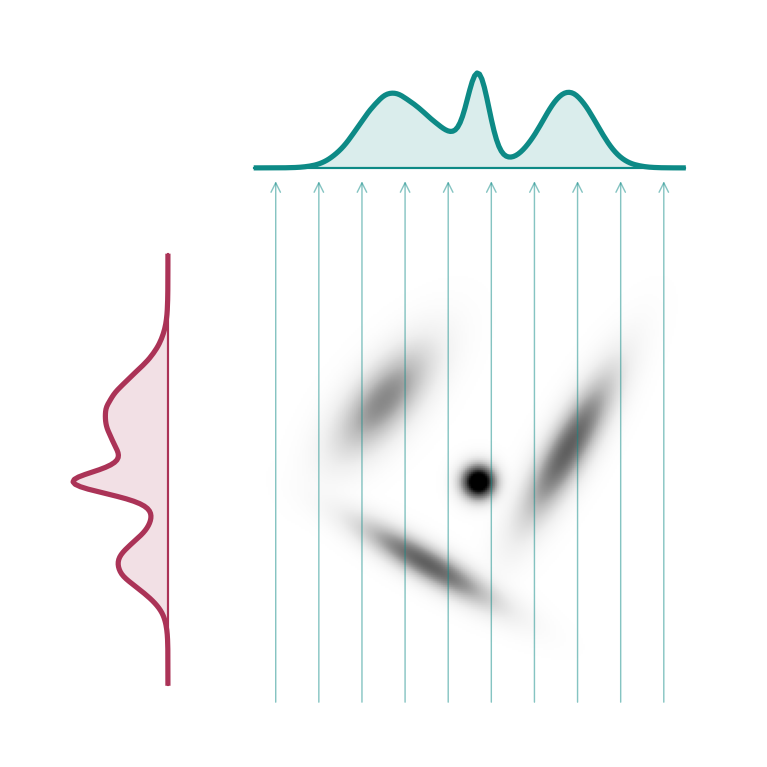
\includegraphics[width=0.95\linewidth]{figs/tomo_projections.png}

\scriptsize a density in $\R^2$ (grey) and two of its projections:
integrate along the rays, record the profile
\column{0.56\textwidth}
\small
An image is a point $x\in\R^N$; natural images have a density $p(x)$.
A filter response $z=\inner{h}{x}$ \emph{projects} $x$ onto the direction $h$. Its histogram is
\begin{keybox}
\[
\rho_h(t)=\int p(x)\,\delta\big(t-\inner{h}{x}\big)\,dx\;=\;(\mathcal R p)(h,t),
\]
the \textbf{Radon transform} of the density along $h$.
\end{keybox}
\begin{itemize}\small
\item All projections together determine $p$ (Cram\'er--Wold).
\item A filter bank $\times$ all shifts $=$ many projection directions; their histograms are
      cheap to measure.
\item \textbf{The tomography question}: rebuild the density --- or rather its potential
      $-\log p$ --- from its projections.
\end{itemize}
\end{columns}
\end{frame}

\begin{frame}{Maximum entropy turns projections into a fields of experts \hfill\tagold}
\begin{columns}[T]
\column{0.55\textwidth}
\small
Among all densities with the measured projections, take the one with maximum entropy:
\[
\max_q\ H(q)\quad\text{s.t.}\quad (\mathcal R q)(h_k,\cdot)=\rho_k\ \ \forall k .
\]
The Lagrange multipliers are whole functions $\varphi_k$, and the solution is
\begin{keybox}
\[
q(x)\;\propto\;\exp\Big(\sum_k\varphi_k\big(\inner{h_k}{x}\big)\Big)
\]
and with convolution filters (all shifts): $\ \log q(x)=\sum_{k,i}\varphi_k\big((h_k*x)_i\big)+\text{const}$.
\end{keybox}
That is exactly a \textbf{fields-of-experts} prior, with potentials $\lambda_k=-\varphi_k$.
\column{0.42\textwidth}
\small
\textbf{Back-projection.} In tomography, $(\mathcal R^*g)(x)=\sum_k g_k(\inner{h_k}{x})$:
a sum of ridge functions. So the log-density is the \emph{back-projection} of the $\varphi_k$.

\medskip
\textbf{Which $\varphi_k$?} The naive choice back-projects the log-histograms:
$\varphi_k=\log\rho_k$ (product of marginals).

\medskip
\begin{oldbox}
\scriptsize FRAME (Zhu, Wu, Mumford 1998): max-entropy with filter histograms, fitted by Gibbs
sampling. Exact fit: iterative proportional fitting (Deming--Stephan 1940). Projection pursuit
density estimation (Friedman et al.\ 1984).
\end{oldbox}
\end{columns}
\end{frame}

\begin{frame}{Unfiltered back-projection over-counts; one linear solve fixes it (2-D testbed)}
\centering
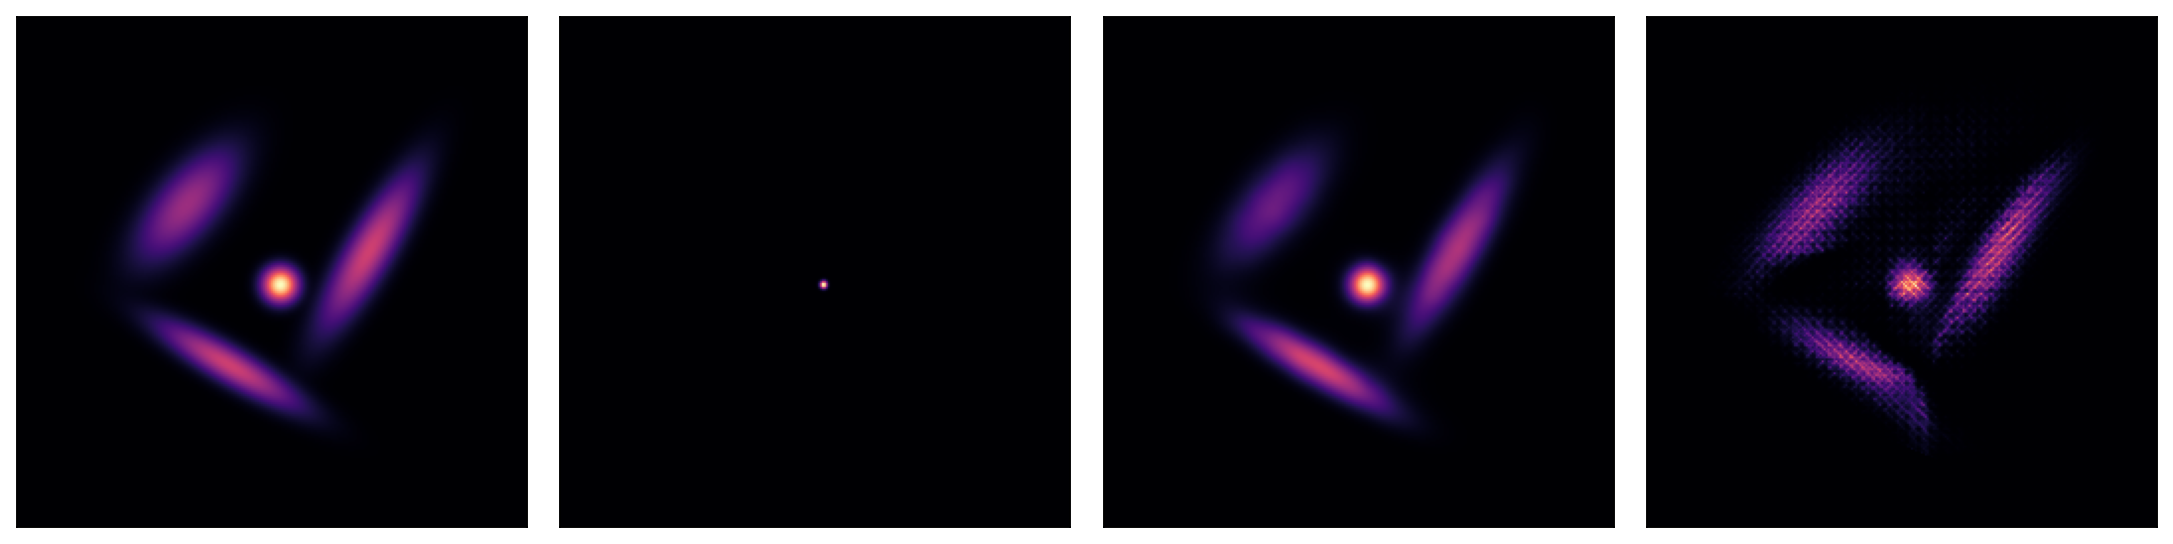
\includegraphics[width=0.96\linewidth]{figs/tomo_recon.png}\\[-1mm]
\footnotesize
\begin{tabular}{@{}*{4}{>{\centering\arraybackslash}p{0.235\linewidth}}@{}}
target density & \textcolor{wine}{\textbf{unfiltered}}: each direction alone & \textcolor{teal}{\textbf{filtered}}: one linear solve $Ac=d$ & iterative max-entropy (IPF, 2 sweeps)\\
 & KL $=39.5$ & KL $=\mathbf{0.03}$ & KL $=0.25$\\
\end{tabular}

\medskip
\begin{keybox}
\small 64 directions in $\R^2$, so every direction overlaps its neighbours (redundancy $\kappa=K/N=32$).
Model: $\log q(x)=\sum_k\varphi_k(\inner{\theta_k}{x})$, fitted by score matching --- the same normal
equations as for images. \textbf{Unfiltered} = keep only the diagonal blocks of $A$ (each direction fitted
alone, $\approx$ log-histograms): information counted $\approx\kappa$ times, the model collapses.
\textbf{Filtered} = the full solve: the overlap is undone and the density is recovered.
\end{keybox}
\end{frame}

\begin{frame}{Testbed: marginals and potentials}
\centering
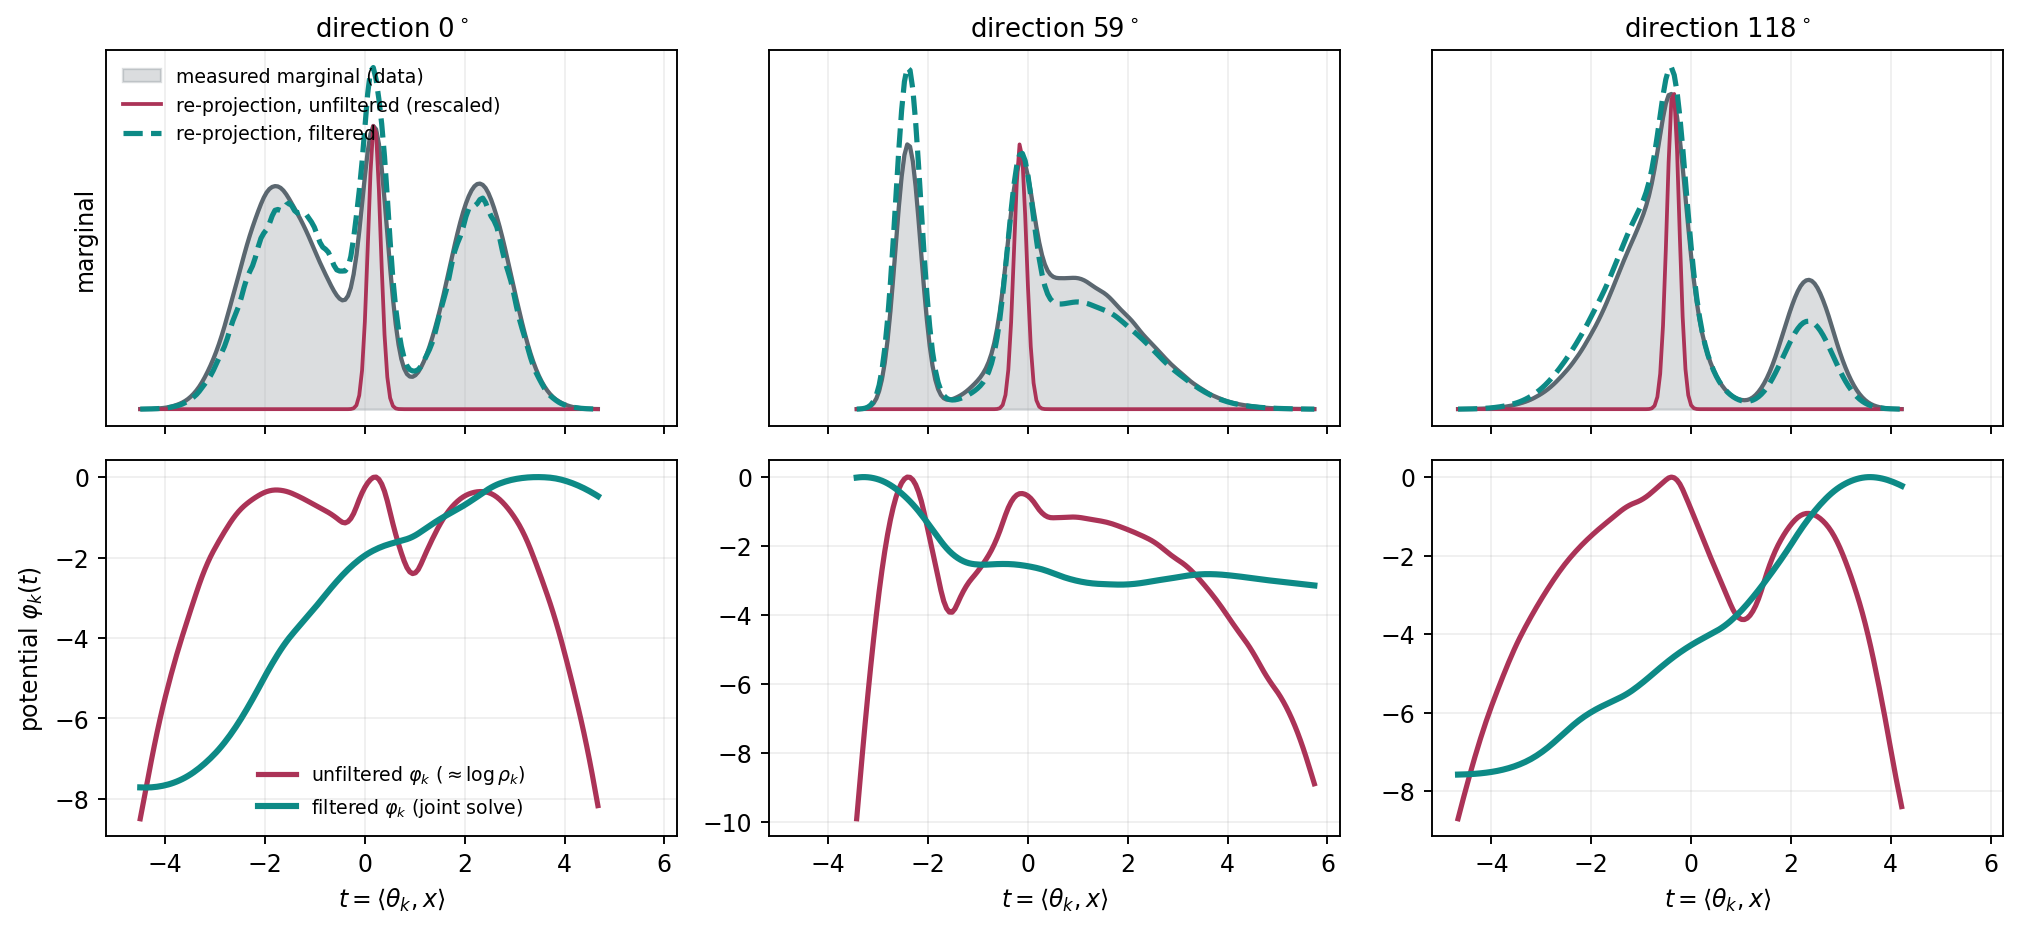
\includegraphics[width=0.86\linewidth]{figs/tomo_marg_pot.png}

\footnotesize\raggedright
\textbf{Top} (tomographic check): projecting each fitted model back onto a direction. The \textcolor{teal}{filtered}
model reproduces the measured marginal; the \textcolor{wine}{unfiltered} one collapses to a spike.\\
\textbf{Bottom}: unfiltered potentials are the log-histograms. Filtered potentials are \emph{shares}: smoother,
and they trade tilts and curvature with the other directions, so only their sum is meaningful.
\end{frame}

\begin{frame}{Score matching \emph{is} filtered back-projection, in closed form \hfill\tagnew}
\begin{columns}[T]
\column{0.5\textwidth}
\small
The normal equations $A\,c=d$ of the next section split exactly like a tomographic
reconstruction:
\begin{itemize}\small
\item $d_{(k,a)}=\E\sum_i b_a'(z_{k,i})$ (Stein's lemma) uses \textbf{only the histogram of
      channel $k$}: the back-projected data.
\item $A_{(k,a),(l,b)}=\E\inner{h_k^\top*b_a(z_k)}{h_l^\top*b_b(z_l)}$ measures how the projection
      directions \textbf{overlap}: the normal operator, like $\mathcal R^*\mathcal R$ in CT.
\item $c=A^{-1}d$: \textbf{filtered} back-projection. Keep only the diagonal blocks of $A$ and
      you get the per-channel (marginal) potentials: \textbf{unfiltered}.
\end{itemize}
\column{0.48\textwidth}
\footnotesize
\renewcommand{\arraystretch}{1.12}
\begin{tabular}{@{}>{\raggedright\arraybackslash}p{2.5cm}>{\raggedright\arraybackslash}p{3.5cm}@{}}
\toprule
tomography (CT) & image priors (here)\\\midrule
object $f$ & potential $-\log p$ of images\\
angle $\theta$ & filter $h_k$ (and its shifts)\\
projection $\mathcal R_\theta f$ & histogram of $h_k*x$\\
back-projection $\mathcal R^*g$ & $\sum_{k,i}\varphi_k((h_k*x)_i)$ (FoE)\\
unfiltered BP: blurred & product of marginals: over-counted ($\beta^\star\approx\bcal/230$)\\
ramp filter $|\omega|$ & $A^{-1}$: undo the overlap\\
iterative (ART) & IPF: exact max-entropy\\
FBP, closed form & one linear solve\\
\bottomrule
\end{tabular}
\end{columns}

\medskip
\begin{keybox}
\small In images the ``ramp filter'' is not a fixed $|\omega|$: $A$ is measured from data, so it is the
exact correction for this bank and this model class. The rest of the talk: which density to
reconstruct (the \emph{noisy} one), and how to turn it into MAP potentials.
\end{keybox}
\end{frame}

% =====================================================================
\begin{frame}{Notation (everything else is built from this)}
\begin{columns}[T]
\column{0.5\textwidth}
\textbf{Data}
\begin{itemize}
\item clean image $x\in[0,1]^{N}$, noisy $y=x+\sigma n$, $n\sim\mathcal N(0,I)$
\item $\sigma=25/255$ throughout
\item filters $h_1,\dots,h_K$: zero mean, $\|h_k\|=1$; responses $z_k=h_k*x$
\item $h_k^\top*$ : the adjoint (correlation) of $h_k*$
\end{itemize}
\textbf{Densities}
\begin{itemize}
\item $p$: density of clean images; $p_\sigma=p*\mathcal N(0,\sigma^2 I)$: noisy images
\item $\rho_k$: marginal density of one response $z_{k,i}$
\end{itemize}
\column{0.5\textwidth}
\textbf{Model class} (two kinds of experts)
\[
R(x)=\underbrace{\sum_{k,i}\lambda_k(z_{k,i})}_{\text{1-D experts}}
+\underbrace{\sum_{k,i}\tfrac1m F_k\!\big(\log A_{k,i}\big)}_{\text{scale field}}
\]
$A_{k,i}=\sum_{j\in\text{window}(i)} z_{k,j}^2/s_k^2$: local energy of filter $k$
in a $(2r+1)^2$ window, $m=(2r+1)^2$.

\medskip
\textbf{Units.} A penalty is drawn in \emph{data-term units}, i.e.\ as $\beta\lambda_k$:
what is added to $\tfrac12\|x-y\|^2$. Then ours and WCRR's are directly comparable.
\end{columns}
\end{frame}

% =====================================================================
\begin{frame}{What is trained, what is explicit}
\centering
\renewcommand{\arraystretch}{1.12}
\footnotesize
\begin{tabular}{@{}p{2.6cm}p{4.3cm}p{6.1cm}@{}}
\toprule
ingredient & WCRR & ours\\\midrule
filters $h_k$ & \TRN{trained} (bilevel, deep equilibrium) &
  \emph{given}: WCRR's own 60 (like-for-like test), or V4 = DCT + steerable pyramid (\EXP{analytic})\\
1-D potentials $\lambda_k$ & \TRN{trained} spline, weakly convex by design & \EXP{explicit}: one linear least-squares solve\\
scale-field term $F_k$ & --- & \EXP{explicit}: same linear solve\\
weight $\beta$ & \TRN{trained} noise-dependent scaling & \EXP{predicted} $\beta=\sigma^2$ (or 1 scalar \HLD{tuned} on 16 images)\\
ridge / roughness & (training choices) & \HLD{chosen} on 44 held-out images, same objective\\
data & BSD400 crops & the same BSD400 crops\\
cost & $\approx$\,3.0\,h on a V100 (measured) & 2.8\,min on the same GPU type, 3 linear solves\\
\bottomrule
\end{tabular}

\medskip
\EXP{teal} = closed form \quad \TRN{wine} = trained by gradient descent \quad
\HLD{amber} = chosen on held-out training images. \emph{No test image is ever used.}
\end{frame}

% =====================================================================
\begin{frame}{The whole method on one page}
\centering
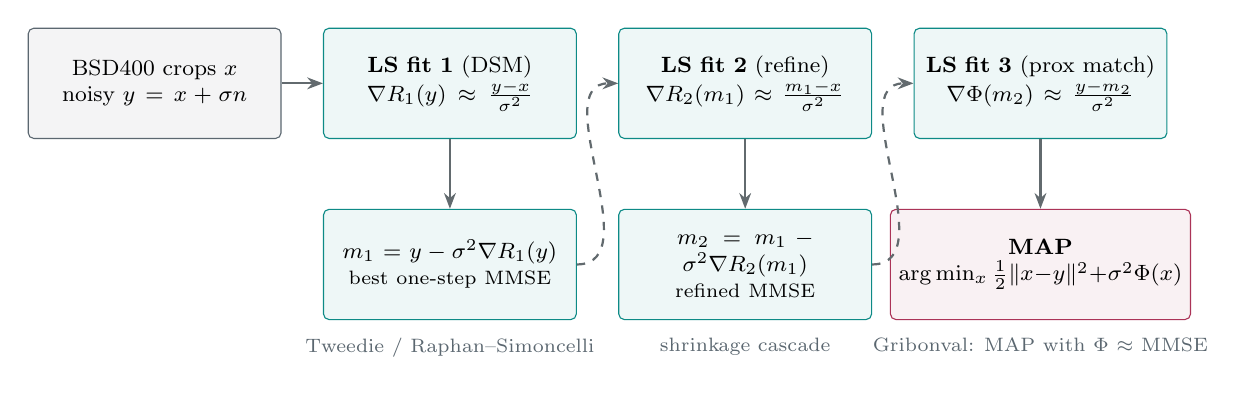
\begin{tikzpicture}
\node[box=slate] (d) at (0,0) {BSD400 crops $x$\\ noisy $y=x+\sigma n$};
\node[box=teal] (s1) at (3.75,0) {\textbf{LS fit 1} (DSM)\\ $\nabla R_1(y)\approx\frac{y-x}{\sigma^2}$};
\node[box=teal] (s2) at (7.5,0) {\textbf{LS fit 2} (refine)\\ $\nabla R_2(m_1)\approx\frac{m_1-x}{\sigma^2}$};
\node[box=teal] (px) at (11.25,0) {\textbf{LS fit 3} (prox match)\\ $\nabla\Phi(m_2)\approx\frac{y-m_2}{\sigma^2}$};
\node[box=teal] (m1) at (3.75,-2.3) {$m_1=y-\sigma^2\nabla R_1(y)$\\ \scriptsize best one-step MMSE};
\node[box=teal] (m2) at (7.5,-2.3) {$m_2=m_1-\sigma^2\nabla R_2(m_1)$\\ \scriptsize refined MMSE};
\node[box=wine,text width=36mm] (map) at (11.25,-2.3) {\textbf{MAP}\\ $\arg\min_x\tfrac12\|x-y\|^2+\sigma^2\Phi(x)$};
\draw[arr] (d)--(s1); \draw[arr] (s1)--(m1); \draw[arr] (s2)--(m2); \draw[arr] (px)--(map);
\draw[arr,dashed] (m1.east) to[out=0,in=180] (s2.west);
\draw[arr,dashed] (m2.east) to[out=0,in=180] (px.west);
\node[lab,below=1mm of m1] {Tweedie / Raphan--Simoncelli};
\node[lab,below=1mm of m2] {shrinkage cascade};
\node[lab,below=1mm of map] {Gribonval: MAP with $\Phi$ $\approx$ MMSE};
\end{tikzpicture}

\medskip
\begin{keybox}
Every box in teal is \textbf{the same routine}: least squares for a gradient field that is
\emph{linear in the coefficients}, evaluated at some points $p$, matched to some target $t$.
Only the pair $(p,t)$ changes.
\end{keybox}
\end{frame}

% =====================================================================
\section{Three classical facts}

\begin{frame}{Fact 1 --- Tweedie: the best denoiser is one gradient step \hfill\tagold}
\begin{columns}[T]
\column{0.56\textwidth}
For Gaussian noise, the posterior mean (MMSE estimator) is
\begin{keybox}
\[
\E[x\mid y]=y+\sigma^2\,\nabla\log p_\sigma(y).
\]
\end{keybox}
\small (Robbins 1956, Miyasawa 1961, Efron 2011.) One line of proof:
$\nabla p_\sigma(y)=\int \frac{x-y}{\sigma^2}\,p(y|x)p(x)\,dx$, divide by $p_\sigma(y)$.

\medskip
\textbf{Reading.} If we knew the \emph{noisy}-image density $p_\sigma$, the optimal
denoiser would be a single gradient step on $\log p_\sigma$ from $y$, with step $\sigma^2$.
\column{0.4\textwidth}
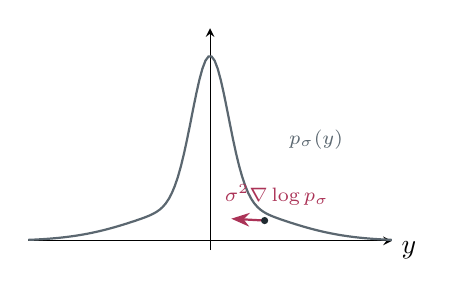
\begin{tikzpicture}
\begin{axis}[width=6.2cm,height=4.4cm,axis lines=middle,xmin=-3,xmax=3,ymin=-0.05,ymax=1.15,
  xtick=\empty,ytick=\empty,xlabel={$y$},every axis x label/.style={at={(1,0)},anchor=west}]
\addplot[slate,thick,domain=-3:3,samples=120] {0.8*exp(-x^2/0.18)+0.2*exp(-x^2/2.5)};
\node[font=\scriptsize,text=slate] at (axis cs:1.75,0.55) {$p_\sigma(y)$};
\draw[-{Stealth},wine,thick] (axis cs:0.9,0.11) -- (axis cs:0.35,0.12);
\node[font=\scriptsize,text=wine] at (axis cs:1.1,0.25) {$\sigma^2\nabla\log p_\sigma$};
\fill[ink] (axis cs:0.9,0.11) circle (1.3pt);
\end{axis}
\end{tikzpicture}
\end{columns}
\end{frame}

\begin{frame}{Fact 2 --- Denoising score matching is plain regression \hfill\tagold}
Choose $R$ to make the one-step denoiser $y-\sigma^2\nabla R(y)$ as good as possible.
Its error is
\[
\E\big\|\,(y-\sigma^2\nabla R(y))-x\,\big\|^2
=\sigma^4\;\E\Big\|\nabla R(y)-\frac{y-x}{\sigma^2}\Big\|^2 .
\]
The right-hand side is \textbf{denoising score matching} (Vincent 2011): regress the gradient
field $\nabla R$ on the target $(y-x)/\sigma^2$ over pairs $(x,y)$. Its minimiser over all
functions is $\nabla R=-\nabla\log p_\sigma$, i.e.\ Tweedie.

\begin{keybox}[title={Two consequences we use}]
\begin{enumerate}
\item Fitting $R$ by DSM \emph{at the noise level of the task} gives the best one-step denoiser
      in the model class --- \EXP{no step size to tune} (it must be exactly $\sigma^2$).
\item The held-out DSM objective $J_{\text{val}}$ \emph{is} the held-out MSE:
      \quad $\text{MSE}_{\text{out}}=\text{MSE}_{\text{in}}+2\sigma^4 J_{\text{val}}$.
      Model selection on $J_{\text{val}}$ = selection on held-out PSNR.
\end{enumerate}
\end{keybox}
\end{frame}

\begin{frame}{Fact 3 --- The MMSE denoiser is itself a MAP estimator \hfill\tagold}
\begin{columns}[T]
\column{0.53\textwidth}
\small
$D(y)=\E[x|y]=\nabla\psi(y)$ with $\psi(y)=\tfrac12\|y\|^2+\sigma^2\log p_\sigma(y)$, and
\[
\nabla^2\psi(y)=\operatorname{Cov}[x\mid y]/\sigma^2\succeq0 .
\]
So $D$ is the gradient of a \emph{convex} function. Gribonval (2011) and Gribonval--Nikolova
(2020): then $D$ is a proximal operator,
\begin{keybox}
\[
D(y)=\arg\min_x\ \tfrac12\|x-y\|^2+\sigma^2\Phi(x),
\]
with $\sigma^2\Phi+\tfrac12\|\cdot\|^2$ convex (\textbf{weakly convex} $\Phi$).
\end{keybox}
\textbf{Reading.} MAP with the true prior $-\log p$ is \emph{not} optimal. MAP with $\Phi$ is.
$\Phi\neq-\log p$: it is smoother. Its weak convexity is exactly the constraint WCRR builds in.
\column{0.45\textwidth}
\centering{\scriptsize 1-D toy: sparse prior, $\sigma=1$}\\[1mm]
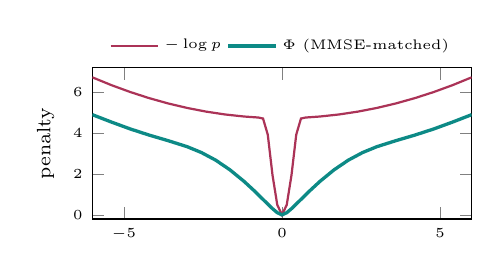
\begin{tikzpicture}
\begin{axis}[width=6.4cm,height=3.5cm,xmin=-6,xmax=6,ymin=-0.2,ymax=7.2,
  ylabel={\scriptsize penalty},
  tick label style={font=\tiny},legend style={font=\tiny,at={(0.5,1.02)},anchor=south,draw=none,fill=none},
  legend columns=2]
\addplot[wine,thick] coordinates {(-6.00,6.739) (-5.40,6.359) (-4.80,6.019) (-4.20,5.719) (-3.60,5.459) (-3.00,5.239) (-2.40,5.059) (-1.80,4.919) (-1.20,4.819) (-0.75,4.770) (-0.60,4.721) (-0.45,3.929) (-0.30,1.946) (-0.15,0.494) (0.00,0.000) (0.15,0.494) (0.30,1.946) (0.45,3.929) (0.60,4.721) (0.75,4.770) (1.20,4.819) (1.80,4.919) (2.40,5.059) (3.00,5.239) (3.60,5.459) (4.20,5.719) (4.80,6.019) (5.40,6.359) (6.00,6.739)};
\addlegendentry{$-\log p$}
\addplot[teal,very thick] coordinates {(-6.00,4.910) (-5.40,4.550) (-4.80,4.210) (-4.20,3.908) (-3.60,3.635) (-3.00,3.341) (-2.55,3.055) (-2.10,2.683) (-1.65,2.211) (-1.20,1.641) (-0.90,1.212) (-0.60,0.757) (-0.30,0.305) (-0.15,0.108) (0.00,0.000) (0.15,0.108) (0.30,0.305) (0.60,0.757) (0.90,1.212) (1.20,1.641) (1.65,2.211) (2.10,2.683) (2.55,3.055) (3.00,3.341) (3.60,3.635) (4.20,3.908) (4.80,4.210) (5.40,4.550) (6.00,4.910)};
\addlegendentry{$\Phi$ (MMSE-matched)}
\end{axis}
\end{tikzpicture}
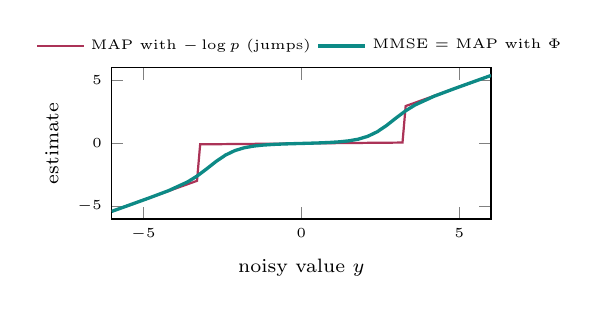
\begin{tikzpicture}
\begin{axis}[width=6.4cm,height=3.5cm,xmin=-6,xmax=6,ymin=-6,ymax=6,
  ylabel={\scriptsize estimate},xlabel={\scriptsize noisy value $y$},
  tick label style={font=\tiny},legend style={font=\tiny,at={(0.5,1.02)},anchor=south,draw=none,fill=none},
  legend columns=2]
\addplot[wine,thick] coordinates {(-6.00,-5.400) (-5.00,-4.500) (-4.00,-3.600) (-3.30,-2.970) (-3.20,-0.070) (-2.00,-0.045) (-1.00,-0.022) (0.00,0.000) (1.00,0.022) (2.00,0.045) (3.20,0.070) (3.30,2.970) (4.00,3.600) (5.00,4.500) (6.00,5.400)};
\addlegendentry{MAP with $-\log p$ (jumps)}
\addplot[teal,very thick] coordinates {(-6.00,-5.400) (-5.40,-4.860) (-4.80,-4.317) (-4.20,-3.752) (-3.60,-3.061) (-3.30,-2.595) (-3.00,-2.030) (-2.70,-1.436) (-2.40,-0.926) (-2.10,-0.565) (-1.80,-0.339) (-1.50,-0.206) (-1.20,-0.128) (-0.90,-0.079) (-0.60,-0.046) (-0.30,-0.021) (0.00,0.000) (0.30,0.021) (0.60,0.046) (0.90,0.079) (1.20,0.128) (1.50,0.206) (1.80,0.339) (2.10,0.565) (2.40,0.926) (2.70,1.436) (3.00,2.030) (3.30,2.595) (3.60,3.061) (4.20,3.752) (4.80,4.317) (5.40,4.860) (6.00,5.400)};
\addlegendentry{MMSE $=$ MAP with $\Phi$}
\end{axis}
\end{tikzpicture}
\end{columns}
\end{frame}

% =====================================================================
\section{The machinery: one least-squares problem}

\begin{frame}{Linear in the coefficients $\Rightarrow$ one linear solve}
Expand each potential's derivative on a fixed basis (hat functions on log-spaced knots):
\[
\lambda_k'(z)=\psi_k(z)=\operatorname{sign}(z)\sum_{a=1}^{29}c_{k,a}\,b_a\!\big(|z|/c_k\big),
\qquad F_k'(L)=\sum_{a=1}^{16}e_{k,a}\,g_a(L).
\]
Then the gradient of the whole energy is a \textbf{linear combination of fixed images}:
\[
\nabla R(p)=\sum_j c_j\,G_j(p),\qquad
G_{(k,a)}(p)=h_k^\top*\big[b_a(h_k*p)\big]\quad(\text{and similarly for the scale field}).
\]
\begin{keybox}[title={Normal equations}]
\[
\min_c\ \E\Big\|\sum_j c_jG_j(p)-t\Big\|^2
\;\Longleftrightarrow\;
\underbrace{\E\inner{G_i(p)}{G_j(p)}}_{A_{ij}}\,c_j=\underbrace{\E\inner{G_i(p)}{t}}_{d_i}
\]
\small 60 filters: $D=60\times(29+16)=2700$ unknowns; $A$ accumulated over 340 crops
($\approx$\,8.8\,M pixels) on the GPU in float64, then $(A+\text{ridge}+\text{roughness})\,c=d$.
\end{keybox}
\end{frame}

\begin{frame}{The three fits are one routine with three (points, target) pairs}
\centering
\renewcommand{\arraystretch}{1.5}
\begin{tabular}{@{}llll@{}}
\toprule
fit & points $p$ & target $t$ & what it gives\\\midrule
1. DSM step & $y$ & $\dfrac{y-x}{\sigma^2}$ & $R_1\approx-\log p_\sigma$; $\;m_1=y-\sigma^2\nabla R_1(y)$ (Tweedie)\\
2. refinement step & $m_1$ & $\dfrac{m_1-x}{\sigma^2}$ & $m_2=m_1-\sigma^2\nabla R_2(m_1)$ (better MMSE estimate)\\
3. prox matching & $m_2$ & $\dfrac{y-m_2}{\sigma^2}$ & $\Phi$ with $\operatorname{prox}_{\sigma^2\Phi}(y)\approx m_2$: \textbf{the MAP potentials}\\
\bottomrule
\end{tabular}

\bigskip
\begin{columns}[T]
\column{0.48\textwidth}
\begin{oldbox}[title={Why fit 3 is the right target}]
MAP optimality of $\hat x$: \ $y-\hat x=\sigma^2\nabla\Phi(\hat x)$.\\
We want $\hat x=$ MMSE estimate $m_2$. So $\nabla\Phi$ must map $m_2\mapsto(y-m_2)/\sigma^2$:
a regression, linear in $\Phi$'s coefficients.
\end{oldbox}
\column{0.48\textwidth}
\begin{keybox}[title={Consequence}]
MAP with $\Phi$ is run at $\beta=\sigma^2=\bcal$, the Bayesian weight. \textbf{Nothing to tune}.
Measured optimum on held-out images: $1.06\,\bcal$.
\end{keybox}
\end{columns}
\end{frame}

% =====================================================================
\section{Filtered vs unfiltered}

\begin{frame}{Unfiltered vs filtered on images: who owns the evidence?}
\begin{columns}[T]
\column{0.56\textwidth}
\textbf{Unfiltered} (marginals): $\lambda_k=-\log\rho_k$, each filter alone.
Filters overlap: they see the same pixels. Each one claims the full evidence, so it is
counted $\approx$ many times.

\medskip
\textbf{Filtered}: solve the \emph{joint} normal equations. The off-diagonal blocks of $A$
measure how much the gradient fields of two filters overlap; solving $Ac=d$ shares the
evidence among them, like multiple regression with correlated regressors.

\medskip
\begin{keybox}
Over-counting, measured: the unfiltered prior needs $\beta^\star=\mathbf{0.0044}\,\bcal$
($\approx 1/230$). The filtered one: $\beta^\star=\mathbf{1.06}\,\bcal$.
\end{keybox}
\column{0.4\textwidth}
\centering
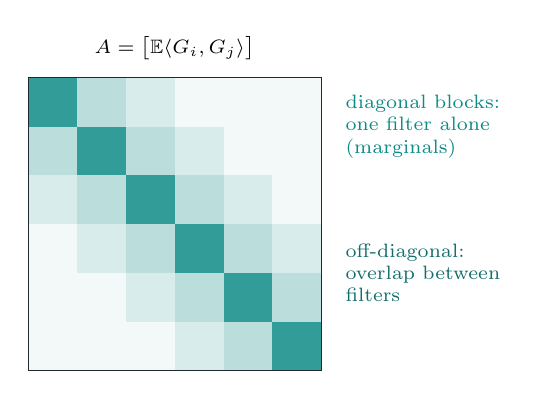
\begin{tikzpicture}[scale=0.62]
\foreach \i in {0,...,5}{\foreach \j in {0,...,5}{
  \pgfmathsetmacro{\v}{\i==\j ? 85 : max(5,40-12*abs(\i-\j))}
  \fill[teal!\v] (\j,-\i) rectangle ++(1,-1);}}
\draw[ink] (0,0) rectangle (6,-6);
\node[font=\scriptsize,align=center] at (3,0.6) {$A=\big[\E\inner{G_i}{G_j}\big]$};
\node[font=\scriptsize,text=teal,align=left,anchor=west] at (6.3,-1) {diagonal blocks:\\ one filter alone\\ (marginals)};
\node[font=\scriptsize,text=teal!70!ink,align=left,anchor=west] at (6.3,-4) {off-diagonal:\\ overlap between\\ filters};
\end{tikzpicture}

\vspace{2mm}
\small Unfiltered $\approx$ keeping only the diagonal.\\ Filtered $=$ the full matrix.
\end{columns}
\end{frame}

\begin{frame}{Calibration: no gain, no $\beta$ to tune --- only when filtered}
\begin{columns}[T]
\column{0.5\textwidth}
\centering\small one-step denoiser $y-g\,\sigma^2\nabla R(y)$, Set12
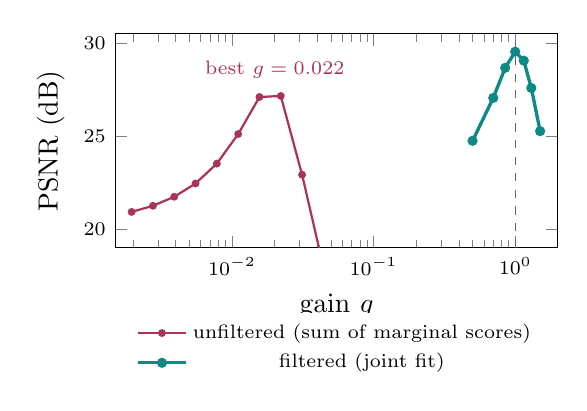
\begin{tikzpicture}
\begin{semilogxaxis}[width=7.2cm,height=4.3cm,xmin=0.0015,xmax=2,ymin=19,ymax=30.5,
  xlabel={gain $g$},ylabel={PSNR (dB)},tick label style={font=\scriptsize},
  legend style={font=\scriptsize,at={(0.5,-0.3)},anchor=north,draw=none},legend columns=1]
\addplot[wine,thick,mark=*,mark size=1pt] coordinates {(0.001953,20.931) (0.002762,21.262) (0.003906,21.745) (0.005524,22.460) (0.007812,23.529) (0.011049,25.115) (0.015625,27.106) (0.022097,27.162) (0.03125,22.928) (0.044194,17.978)};
\addlegendentry{unfiltered (sum of marginal scores)}
\addplot[teal,very thick,mark=*,mark size=1.2pt] coordinates {(0.5,24.752) (0.7,27.058) (0.85,28.675) (1,29.541) (1.15,29.059) (1.3,27.589) (1.5,25.270)};
\addlegendentry{filtered (joint fit)}
\draw[dashed,slate] (axis cs:1,19) -- (axis cs:1,30.5);
\node[font=\scriptsize,text=wine,align=center] at (axis cs:0.02,28.6) {best $g=0.022$};
\end{semilogxaxis}
\end{tikzpicture}
\column{0.5\textwidth}
\centering\small MAP, $\beta$ scan on the 16 tuning images
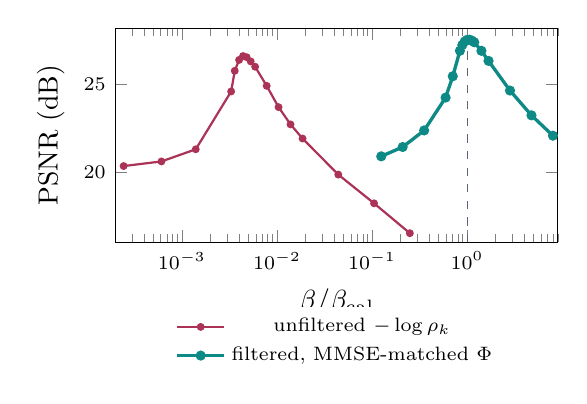
\begin{tikzpicture}
\begin{semilogxaxis}[width=7.2cm,height=4.3cm,xmin=0.0002,xmax=9,ymin=16,ymax=28.2,
  xlabel={$\beta/\bcal$},ylabel={PSNR (dB)},tick label style={font=\scriptsize},
  legend style={font=\scriptsize,at={(0.5,-0.3)},anchor=north,draw=none},legend columns=1]
\addplot[wine,thick,mark=*,mark size=1pt] coordinates {(0.000244,20.344) (0.000610,20.607) (0.0014,21.300) (0.0033,24.597) (0.0036,25.772) (0.0040,26.392) (0.0044,26.614) (0.0048,26.549) (0.0053,26.309) (0.0059,26.004) (0.0078,24.917) (0.0104,23.703) (0.0139,22.718) (0.0186,21.913) (0.0442,19.857) (0.1051,18.220) (0.25,16.517)};
\addlegendentry{unfiltered $-\log\rho_k$}
\addplot[teal,very thick,mark=*,mark size=1.2pt] coordinates {(0.125,20.897) (0.2102,21.430) (0.3536,22.375) (0.5946,24.247) (0.7071,25.462) (0.8409,26.915) (0.8909,27.242) (0.9439,27.441) (1.0,27.537) (1.0595,27.547) (1.1225,27.495) (1.1892,27.400) (1.4142,26.913) (1.6818,26.338) (2.8284,24.647) (4.7568,23.234) (8.0,22.076)};
\addlegendentry{filtered, MMSE-matched $\Phi$}
\draw[dashed,slate] (axis cs:1,16) -- (axis cs:1,28.2);
\end{semilogxaxis}
\end{tikzpicture}
\end{columns}
\small The filtered models peak \textbf{exactly where theory says} ($g=1$, $\beta=\bcal$).
The unfiltered ones need a factor $\approx1/45$ (one step) and $\approx1/230$ (MAP), and still lose $>0.6$\,dB.
\end{frame}

% =====================================================================
\section{Making the potentials interpretable}

\begin{frame}{Redundant filters $\Rightarrow$ per-filter potentials are not identifiable}
\begin{columns}[T]
\column{0.56\textwidth}
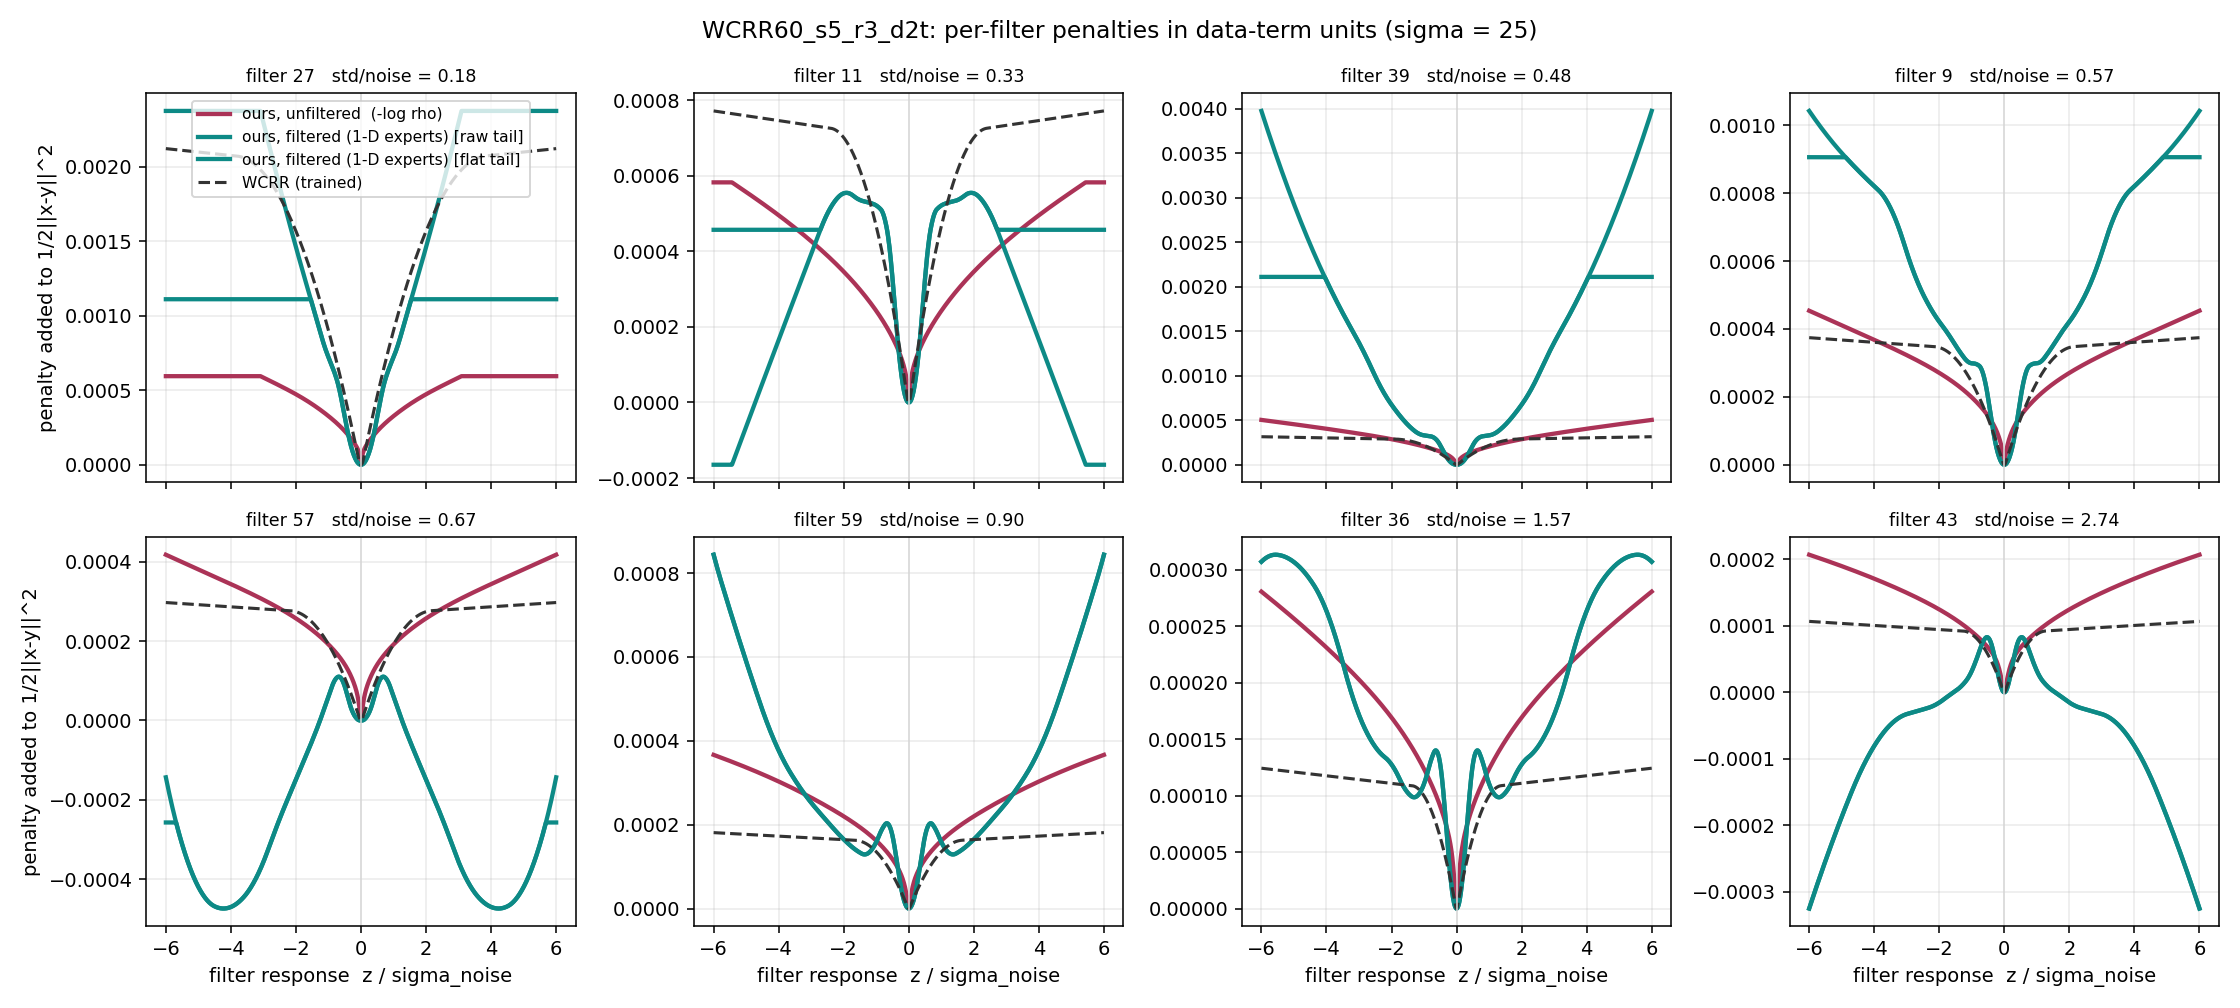
\includegraphics[width=\linewidth]{figs/pot_before.png}

\scriptsize\textbf{Before}: unconstrained fit (earlier pipeline). Wiggles, dips, even negative tails.
\column{0.42\textwidth}
\small
Many combinations of per-filter potentials give almost the same \emph{total} gradient
($A$ has a near-null space). The unconstrained optimum picks an arbitrary one.

\begin{keybox}[title={Shape constraint (convex)}]
$c_{k,a}\ge0$ for all 1-D coefficients\\
$\iff$ each $\lambda_k$ is even and \textbf{non-decreasing in $|z|$} (WCRR's class).\\[2pt]
Box QP $\min_{c\ge0}\tfrac12c^\top Qc-d^\top c$: ADMM (one Cholesky) to find the active set,
then a primal--dual active-set method to the exact KKT point.
\end{keybox}
\footnotesize Costs $0.3\%$ of the held-out objective; MAP on Set12: \textbf{29.17\,$\to$\,29.82} dB.
\end{columns}
\end{frame}

\begin{frame}{The potentials, side by side (WCRR's 60 filters, data-term units)}
\centering
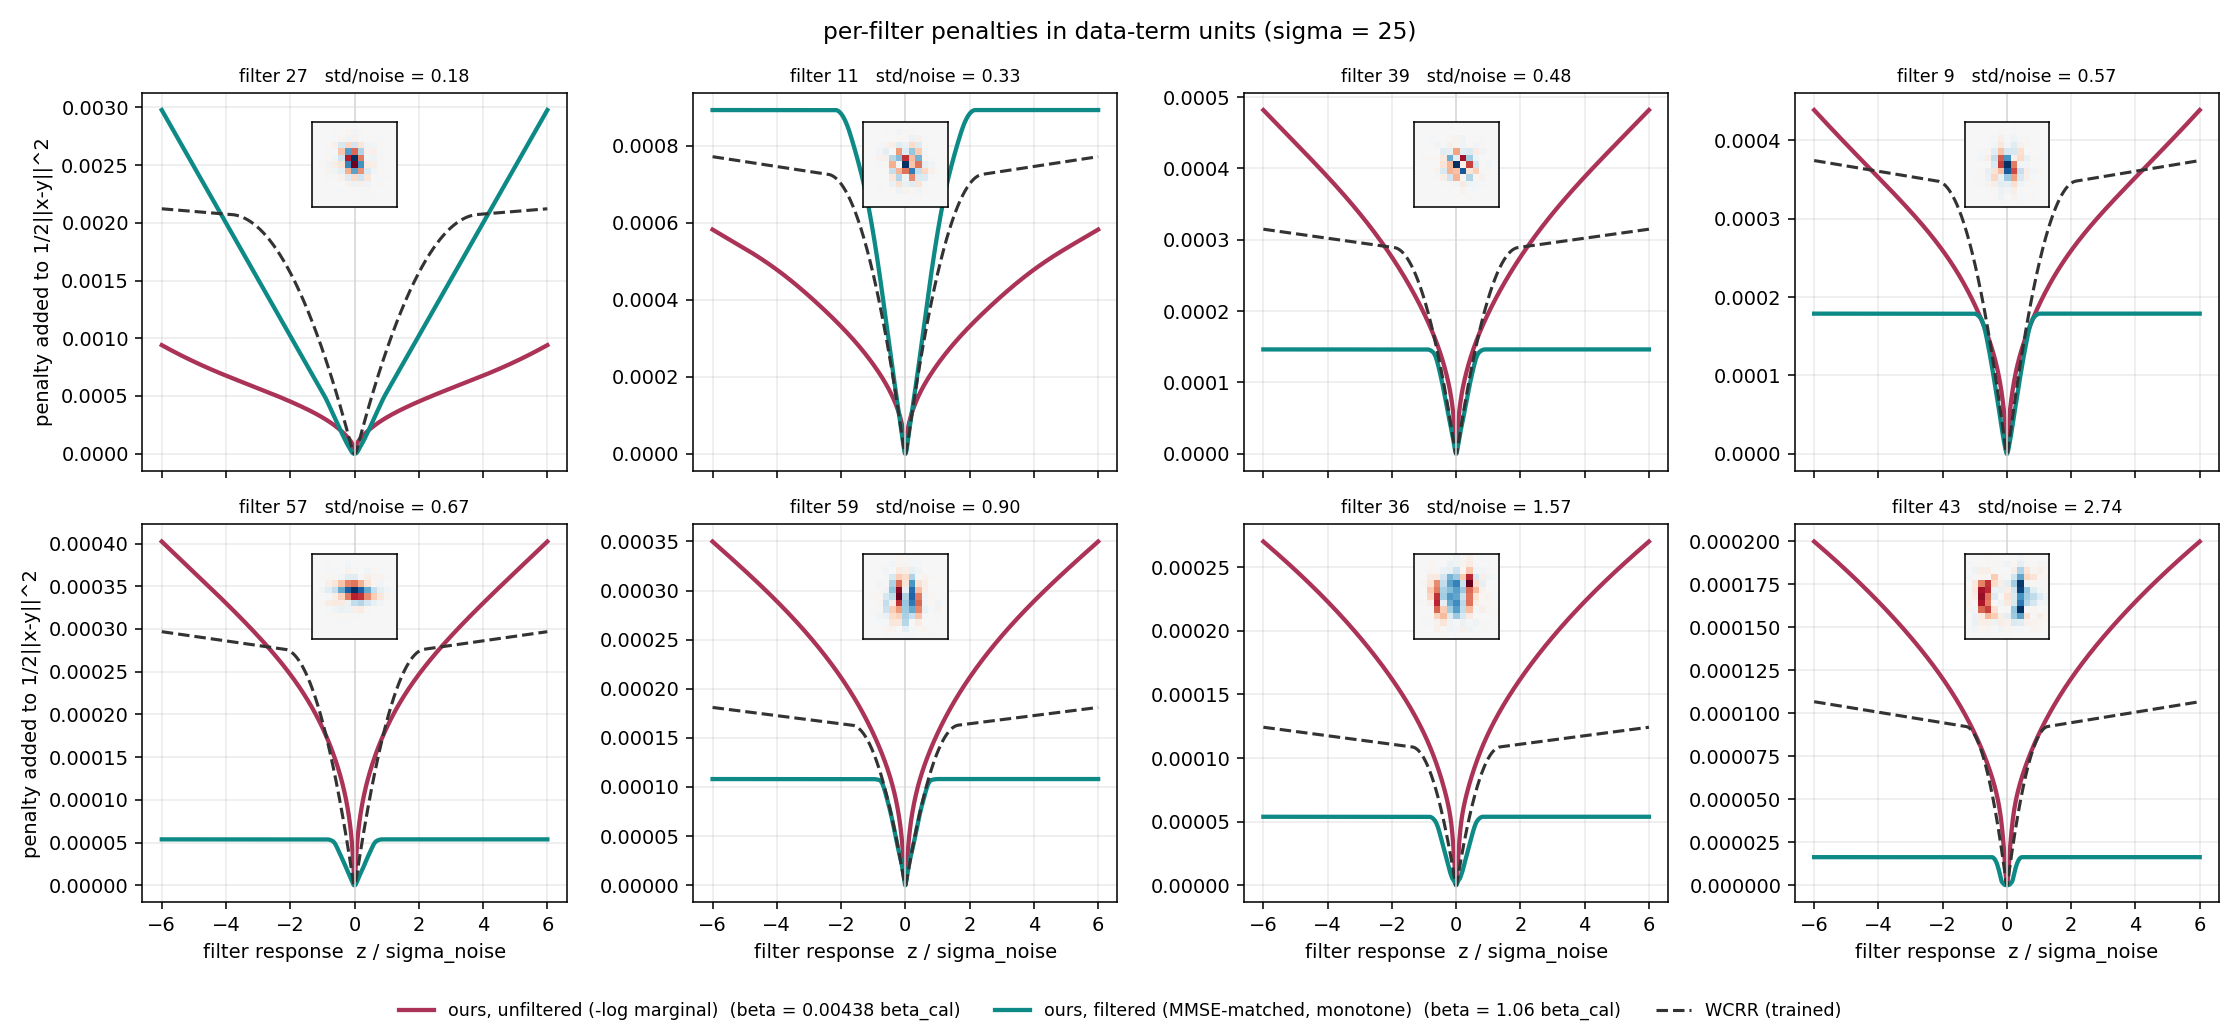
\includegraphics[width=0.92\linewidth]{figs/pot_w60_s25.png}

\footnotesize \textcolor{wine}{Unfiltered}: concave cusps that keep growing (needs $\beta\approx\bcal/230$).
\ \textcolor{teal}{Filtered, MMSE-matched}: quadratic core of width $\approx\sigma$, flat beyond ---
\emph{shrink what looks like noise, leave signal alone}. Dashed: WCRR, trained.
\end{frame}

% =====================================================================
\section{Implementation}

\begin{frame}{Implementation details that matter}
\begin{columns}[T]
\column{0.5\textwidth}
\textbf{Fitting} (\texttt{afoe.py}, $\approx$700 lines, PyTorch)
\begin{itemize}\small
\item responses and adjoints by FFT; feature images in chunks of 16 filters
\item $A,d$ accumulated in float64 over the interior (10\,px border) of 340 crops
\item hyper-parameters (ridge, roughness) on 44 \emph{held-out} crops, by $J_{\text{val}}$
\item potentials stored as fine tables ($96\,001$ points) with exact cell slopes: energy and
      gradient are consistent, so line searches are valid
\item data split fixed: 340 fit / 44 select / 16 tune (BSD400); tests never touched
\end{itemize}
\column{0.5\textwidth}
\textbf{MAP solver}
\begin{itemize}\small
\item FISTA with Beck--Teboulle backtracking, momentum restart when the energy rises, batched
\item \alert{bug found}: the exact backtracking test fails on float32 rounding near convergence,
      and one failing image made the whole batch backtrack 40$\times$ per iteration (BSD68 78$\times$
      slower). Fix: compare energies up to $10^{-6}$ relative.
\item converged at 250 iterations (PSNR identical to 4 decimals at 250/500/1000/2000); we use 500
\item reflect padding; noise seeded per (set, image, $\sigma$): every method sees the same noise
\end{itemize}
\end{columns}
\end{frame}

% =====================================================================
\section{Results}

\begin{frame}{Results (1/2): MAP with explicit potentials on WCRR's own 60 filters}
\centering
\footnotesize
\renewcommand{\arraystretch}{1.2}
\begin{tabular}{@{}llcccc@{}}
\toprule
 & & \multicolumn{2}{c}{PSNR (dB), $\sigma=25$} & \multicolumn{2}{c}{\#\,images $>$ WCRR}\\
\cmidrule(lr){3-4}\cmidrule(lr){5-6}
potentials & $\beta$ & Set12 & BSD68 & Set12 & BSD68\\\midrule
WCRR (\TRN{trained}) & \TRN{trained} & \WSt & \WBs & --- & ---\\\midrule
unfiltered $-\log\rho_k$ & \HLD{tuned}: $0.0044\,\bcal$ & 28.985 & 27.873 & 0/12 & 0/68\\
filtered, 1-D only (= WCRR's class) & $\bcal$ & 29.415 & 28.561 & 0/12 & 7/68\\
filtered, 1-D only & \HLD{tuned}: $1.06\,\bcal$ & 29.521 & 28.603 & 3/12 & 9/68\\
filtered, 1-D + scale field & $\bcal$ & \textbf{29.742} & \textbf{28.712} & 11/12 & 36/68\\
filtered, 1-D + scale field & \HLD{tuned}: $1.06\,\bcal$ & \textbf{29.808} & \textbf{28.737} & 12/12 & 43/68\\
\bottomrule
\end{tabular}

\medskip
\begin{keybox}
\small Same filters, same data, same noise realisations; WCRR re-run with the authors' model and
solver. Only the potentials differ: \TRN{trained} vs \EXP{three linear solves}.
\end{keybox}
\end{frame}

\begin{frame}{Results (2/2): explicit estimators without MAP, and other banks}
\centering
\small
\renewcommand{\arraystretch}{1.2}
\begin{tabular}{@{}llcccc@{}}
\toprule
 & & \multicolumn{2}{c}{PSNR (dB), $\sigma=25$} & \multicolumn{2}{c}{\#\,images $>$ WCRR}\\
\cmidrule(lr){3-4}\cmidrule(lr){5-6}
method & filters & Set12 & BSD68 & Set12 & BSD68\\\midrule
BM3D (reference) & --- & 29.984 & 28.616 & 10/12 & 18/68\\
WCRR (\TRN{trained}) & 60 \TRN{trained} & \WSt & \WBs & --- & ---\\\midrule
one closed-form step & WCRR's 60 & 29.536 & 28.576 & & \\
two closed-form steps & WCRR's 60 & 29.770 & 28.702 & 10/12 & 34/68\\
two closed-form steps & V4 (\EXP{analytic}, 311) & 29.664 & 28.658 & 4/12 & 25/68\\
two closed-form steps & WCRR60 + V4 (371) & \textbf{29.922} & \textbf{28.818} & 12/12 & 61/68\\
\bottomrule
\end{tabular}

\medskip
\begin{keybox}
\small No $\beta$, no step size, no tuning: each step is $m\leftarrow m-\sigma^2\nabla R(m)$ with the
fitted $R$. V4 = DCT-8 + steerable pyramids: a filter bank that involves no learning at all.
\end{keybox}
\end{frame}

\begin{frame}{Which filters? Learned, analytic, and data-analytic}
\centering
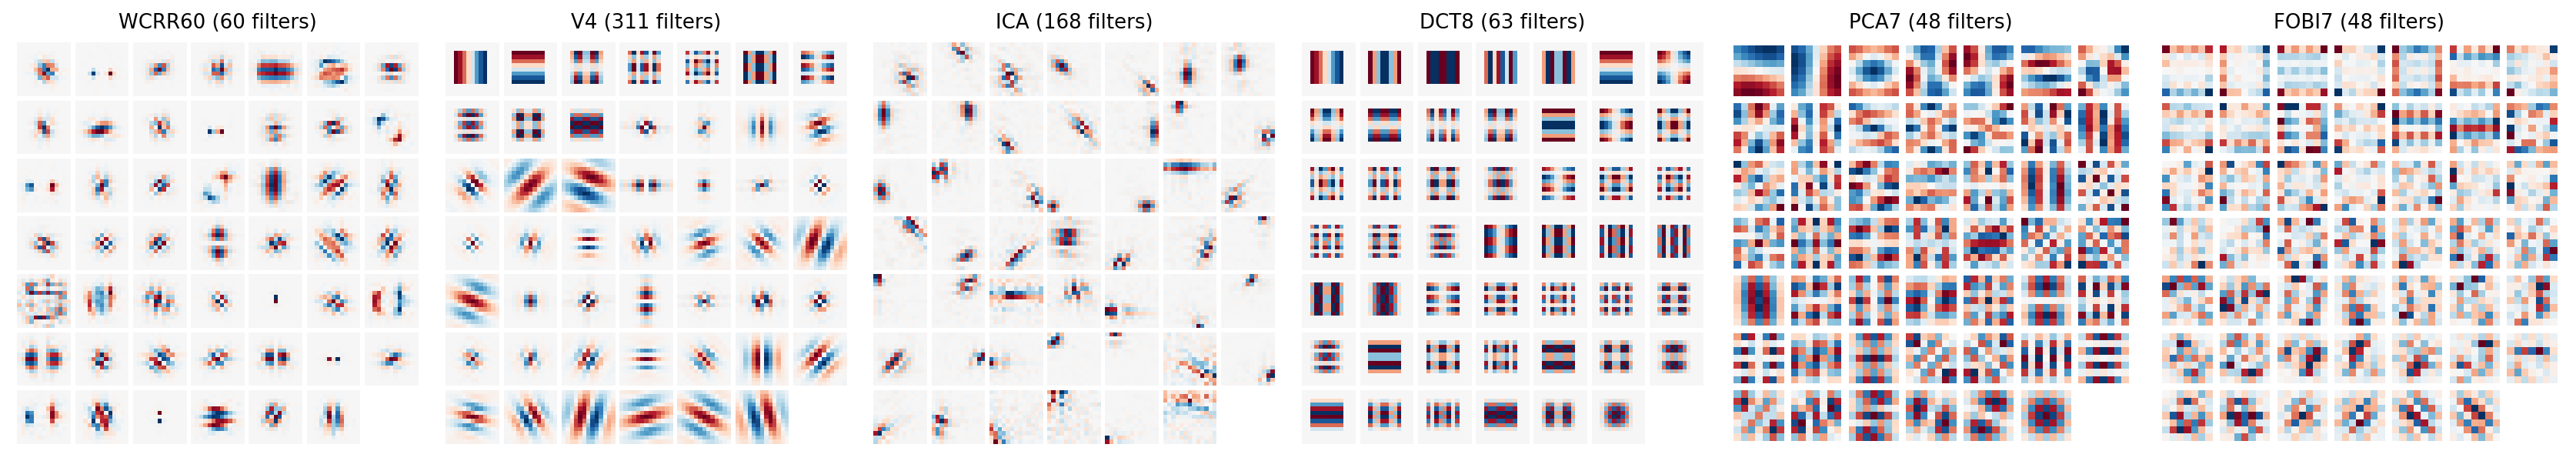
\includegraphics[width=\linewidth]{figs/filters.png}

\vspace{1mm}
\resizebox{0.92\linewidth}{!}{%
\begin{tabular}{@{}llrccc@{}}
\toprule
filters & obtained by & $K$ & held-out (VAL) & Set12 & BSD68\\\midrule
WCRR60 + V4 ($r=5$) & learned + analytic & 371 & 28.05 & 29.92 & 28.82\\
WCRR60 & \TRN{learned} (bilevel training) & 60 & 27.93 & 29.77 & 28.70\\
V4 & \EXP{analytic}: DCT-8 + steerable pyramids & 311 & 27.84 & 29.66 & 28.63\\
ICA $13{\times}13$ & data: FastICA (iterative) & 168 & 27.81 & 29.53 & 28.57\\
PCA $5{\times}5$ & data: patch PCA, \EXP{closed form} & 24 & 27.60 & 29.25 & 28.41\\
DCT $8{\times}8$ & \EXP{analytic} & 63 & 27.59 & 29.32 & 28.40\\
PCA $13{\times}13$ & data: patch PCA, \EXP{closed form} & 168 & 27.44 & 29.12 & 28.27\\
FOBI $5{\times}5$ & data: closed-form ICA & 24 & 27.39 & 28.90 & 28.14\\
\bottomrule
\end{tabular}}

\vspace{1mm}
\scriptsize Two explicit steps, $r=3$, no tuning. \textbf{The held-out objective ranks the banks exactly like the BSD68
test PSNR}: it is the explicit criterion for choosing filters. PCA is optimal only for the Gaussian part; the experts
need localized, oriented filters.
\end{frame}

\begin{frame}{What it looks like (Set12: Monarch, Barbara, Cameraman; zooms)}
\centering
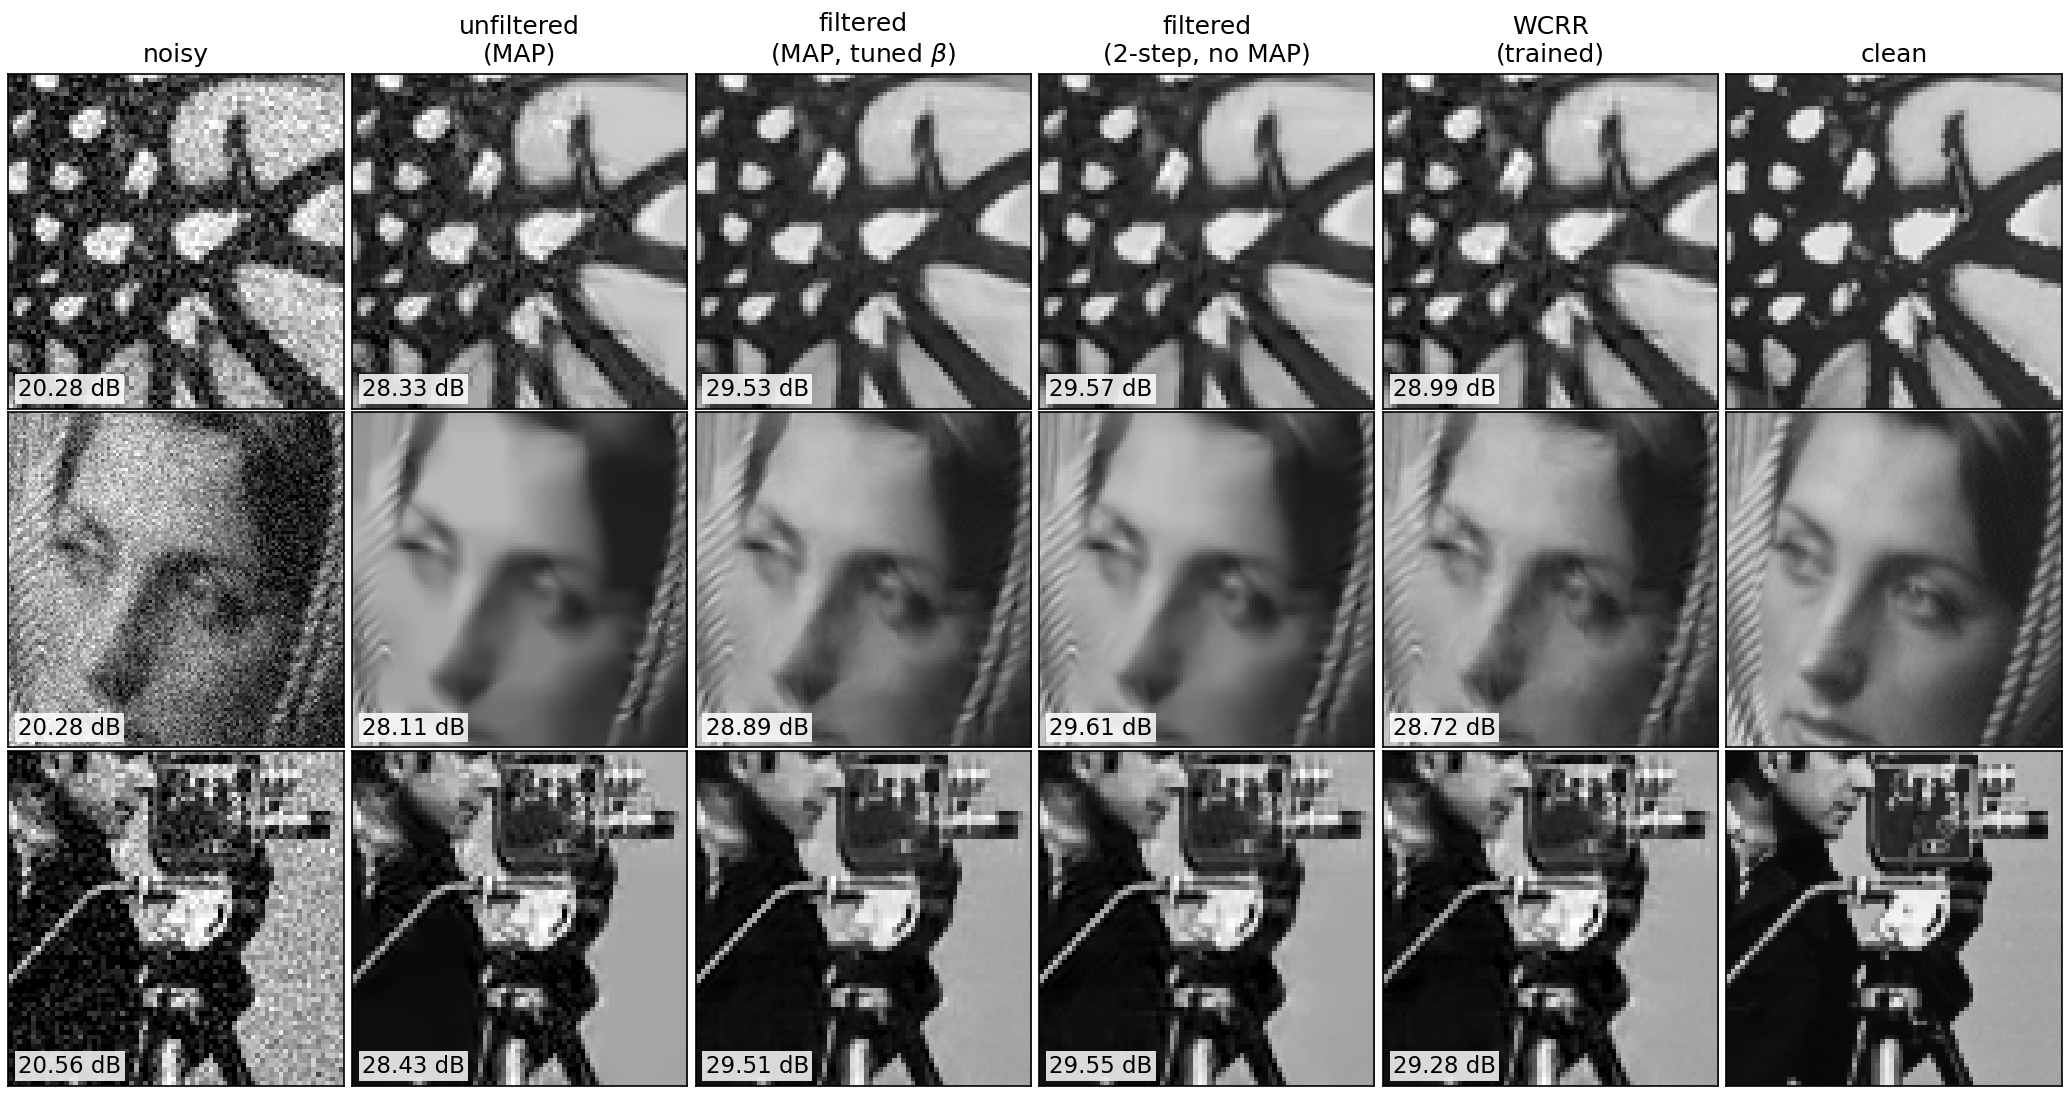
\includegraphics[height=0.78\textheight]{figs/slide_crops.png}

\footnotesize PSNR on the full image. Unfiltered: blotchy noise, erased stripes (over-weighted prior).
Filtered: clean and sharp, texture kept.
\end{frame}

\begin{frame}{Time benchmark (one Tesla V100-SXM2-32GB, same GPU for every row)}
\begin{columns}[T]
\column{0.38\textwidth}
\textbf{Getting the potentials} (from scratch, incl.\ data loading and selection)
\footnotesize
\renewcommand{\arraystretch}{1.15}
\begin{tabular}{@{}lr@{}}
\toprule
\EXP{LS fit 1} (DSM step) & 59.5\,s\\
\EXP{LS fit 2} (refinement step) & 47.3\,s\\
\EXP{LS fit 3} (prox matching) & 60.0\,s\\\midrule
\textbf{ours, total} & \textbf{2.8\,min}\\
WCRR \TRN{training} & \textbf{3.03\,h}\\
\bottomrule
\end{tabular}

\smallskip
\scriptsize WCRR: the repository's own training, measured earlier on a V100: 1.82\,s/batch
$\times$ 6000 batches. Ratio $\approx65\times$.
\column{0.60\textwidth}
\textbf{Denoising one image} (median of 3 runs, after warm-up)
\footnotesize
\renewcommand{\arraystretch}{1.15}
\begin{tabular}{@{}lrr@{}}
\toprule
 & $481\times321$ & $512\times512$\\\midrule
ours: two closed-form steps & \textbf{0.015\,s} & \textbf{0.022\,s}\\
ours: MAP, 1-D + SF, 500 it & 11.7\,s & 17.9\,s\\
ours: MAP, 1-D + SF, 250 it\textsuperscript{*} & 6.0\,s & 9.1\,s\\
ours: MAP, 1-D only, 500 it & 5.5\,s & 7.8\,s\\
unfiltered MAP, 4000 it & 41.7\,s & 59.5\,s\\
WCRR, its own solver & 1.5\,s & 2.2\,s\\
\bottomrule
\end{tabular}

\smallskip
\scriptsize \textsuperscript{*}already converged (same PSNR to 4 decimals as 500--2000 iterations).
\end{columns}

\medskip
\begin{keybox}
\small Fitting is $\approx65\times$ cheaper than training. The explicit two-step denoiser is
$100\times$ faster than WCRR. Our MAP solver is $4$--$8\times$ \emph{slower} than WCRR's (generic
FISTA with line search on tabulated potentials): inference speed is the open engineering item.
\end{keybox}

\end{frame}

% =====================================================================
\section{Interpretation and positioning}

\begin{frame}{How to read the results}
\begin{enumerate}
\item \textbf{Filtering $=$ sharing evidence.} Marginal potentials are right for one filter
      alone; with overlapping filters, the joint least squares divides the evidence.
      The measured over-counting factor ($\beta^\star\approx\bcal/230$) is the price of ignoring it.
\item \textbf{The best MAP prior is not $-\log p$.} The MAP-optimal penalty is the
      MMSE-matched $\Phi$: quadratic up to about the noise level, then saturating. MAP with
      $-\log p$ thresholds hard (the cliff in the $\beta$ scan); MAP with $\Phi$ shrinks smoothly.
\item \textbf{WCRR's design is a theorem.} Weak convexity and the saturating shape, imposed in
      WCRR by architecture, are properties of the exact MMSE-matched penalty.
\item \textbf{$\beta$ is predicted.} $\beta=\sigma^2$ follows from Tweedie; the held-out optimum
      is $1.06\,\bcal$, and using $\bcal$ instead costs 0.03--0.11 dB.
\item \textbf{A local-variance term is what beats WCRR.} In WCRR's exact class (1-D experts,
      same filters) the explicit potentials are 0.08--0.10 dB below; adding the explicit scale
      field puts them 0.03--0.19 dB above (both sets, with or without tuning).
\end{enumerate}
\end{frame}

\begin{frame}{What is \emph{not} new (we build on it)}
\begin{oldbox}[title={Known results used here}]
\small
\begin{itemize}
\item Radon transform, Cram\'er--Wold; maximum entropy with filter histograms (FRAME, Zhu--Wu--Mumford 1998);
      iterative proportional fitting; projection pursuit density estimation.
\item FoE / ridge regularizers: Roth \& Black 2005; Chen \& Pock 2017; WCRR (Goujon et al.\ 2024).
\item Tweedie / Miyasawa formula; score matching (Hyv\"arinen 2005); denoising score matching (Vincent 2011).
\item \textbf{Jointly optimal, linear-in-parameter shrinkage in redundant representations beats
      per-subband (marginal) shrinkage}: Raphan \& Simoncelli 2008 (SURE, per image), Hel-Or \& Shaked
      2008 (supervised). \emph{Our one-step ``filtered vs unfiltered'' result is theirs.}
\item Gaussian scale mixtures / local-variance models: Wainwright \& Simoncelli 2000; Portilla et al.\ 2003
      (and Raphan--Simoncelli's neighbourhood estimators).
\item Cascades of shrinkage stages: Schmidt \& Roth 2014 (shrinkage fields).
\item The MMSE denoiser is the prox of a weakly convex penalty: Gribonval 2011; Gribonval \& Nikolova 2020;
      used for plug-and-play convergence by Hurault et al.\ 2022 (implicit penalty, trained network).
\end{itemize}
\end{oldbox}
\end{frame}

\begin{frame}{What is new here (to be checked against a full literature search)}
\begin{novbox}[title={Methodology}]
\small
\begin{itemize}
\item \textbf{Prox matching as linear least squares}: explicit FoE potentials whose MAP estimate
      reproduces a (closed-form) MMSE estimate --- a MAP regularizer computed, not trained.
\item Reading score matching as \textbf{filtered back-projection in log-density space}: the data term
      is the back-projected histograms, the Gram matrix is the ramp filter (unfiltered = drop its off-diagonal).
\item One routine for everything: DSM, refinement and prox matching differ only by (points, target);
      the held-out objective equals the held-out MSE.
\item A monotone shape constraint (exact box QP) that removes the non-identifiability of potentials in
      redundant banks; it is essential for MAP (29.17\,$\to$\,29.82 dB).
\end{itemize}
\end{novbox}
\begin{novbox}[title={Results and interpretation}]
\small
\begin{itemize}
\item $\beta=\sigma^2$ \emph{predicted} for MAP and confirmed (held-out optimum $1.06\,\sigma^2$).
\item On WCRR's own filters, explicit potentials (+ explicit scale field) \textbf{beat the trained
      potentials on Set12 and BSD68}, without tuning.
\item WCRR's saturating, weakly convex shape is explained (MMSE matching); the over-counting of
      marginal potentials is measured ($\beta^\star\approx\sigma^2/230$).
\end{itemize}
\end{novbox}
\end{frame}

\begin{frame}{Limits and next steps}
\begin{itemize}
\item \textbf{1-D experts alone} (exactly WCRR's class) stay 0.08--0.10 dB below WCRR: the win
      needs the scale-field term.
\item \textbf{Large banks} (V4, union): the fitted scale-field terms \emph{decrease} with local energy
      on 31--48\% of their range (they reward contrast), and the projected MAP becomes unstable
      on high-contrast images (V4: 28.9 dB). Forcing every term to be non-decreasing repairs V4
      (29.42) but costs 0.26 dB on WCRR's filters. Open.
\item Only $\sigma=25$ and denoising so far; the next test is other $\sigma$ and inverse problems
      (deblurring, MRI), where an explicit regularizer is the point.
\item BM3D is still ahead on Set12 (the two-step union estimator: $-0.06$ dB); WCRR's own
      advantage over BM3D is on BSD68, where we now beat both.
\item Novelty claims need a careful literature search, especially around Hurault et al.\ 2022
      and learned proximal networks.
\end{itemize}
\end{frame}

\appendix
\begin{frame}{Backup: what did not work (and why it was informative)}
\small
\begin{itemize}
\item \textbf{DSM at a small noise level, then MAP with tuned $\beta$} (the old route): best 29.37 Set12.
      $\sigma_{\text{fit}}$ sweep 3/4/5/7/10 $\to$ 29.25/29.34/29.37/29.13/28.57. Starting MAP from $y$,
      from the clean image, or from WCRR's output gives the same PSNR: \emph{the energy}, not the
      optimiser, was the limit.
\item \textbf{Per-channel Gribonval transform} of the filtered potentials: 25.1 dB. The MMSE-to-MAP
      conversion must be done jointly (prox matching), not filter by filter.
\item \textbf{Unconstrained prox matching}: 29.17 dB (vs 29.82 monotone).
\item \textbf{Flat tails} beyond the fitted range: collapse (22.0 dB with the scale field).
\item \textbf{More data / knots} (8 flips, 40 knots): no change; larger scale-field window:
      $r=5$ best for the one-step estimator ($+0.035$ dB on BSD68 over $r=3$).
\end{itemize}
\end{frame}

\begin{frame}[allowframebreaks]{References}
\footnotesize
\begin{itemize}
\item J.~Radon. \"Uber die Bestimmung von Funktionen durch ihre Integralwerte l\"angs gewisser Mannigfaltigkeiten. 1917.
\item H.~Cram\'er, H.~Wold. Some theorems on distribution functions. \emph{J.\ London Math.\ Soc.} 1936.
\item S.~C.~Zhu, Y.~N.~Wu, D.~Mumford. Filters, random fields and maximum entropy (FRAME). \emph{IJCV} 1998.
\item J.~H.~Friedman, W.~Stuetzle, A.~Schroeder. Projection pursuit density estimation. \emph{JASA} 1984.
\item W.~E.~Deming, F.~F.~Stephan. On a least squares adjustment of a sampled frequency table. \emph{Ann.\ Math.\ Stat.} 1940.
\item S.~Roth, M.~J.~Black. Fields of Experts. \emph{IJCV} 2009 (CVPR 2005).
\item Y.~Chen, T.~Pock. Trainable nonlinear reaction diffusion. \emph{IEEE TPAMI} 2017.
\item A.~Goujon, S.~Neumayer, M.~Unser. Learning weakly convex regularizers for convergent
      image-reconstruction algorithms. \emph{SIAM J.\ Imaging Sci.} 2024.
\item H.~Robbins 1956; K.~Miyasawa 1961; B.~Efron. Tweedie's formula and selection bias. \emph{JASA} 2011.
\item A.~Hyv\"arinen. Estimation of non-normalized statistical models by score matching. \emph{JMLR} 2005.
\item P.~Vincent. A connection between score matching and denoising autoencoders. \emph{Neural Comput.} 2011.
\item M.~Raphan, E.~P.~Simoncelli. Optimal denoising in redundant representations. \emph{IEEE TIP} 17(8), 2008.
\item Y.~Hel-Or, D.~Shaked. A discriminative approach for wavelet denoising. \emph{IEEE TIP} 2008.
\item M.~Wainwright, E.~Simoncelli. Scale mixtures of Gaussians and the statistics of natural images. \emph{NIPS} 2000.
\item J.~Portilla, V.~Strela, M.~Wainwright, E.~Simoncelli. Image denoising using scale mixtures of Gaussians in the wavelet domain. \emph{IEEE TIP} 2003.
\item U.~Schmidt, S.~Roth. Shrinkage fields for effective image restoration. \emph{CVPR} 2014.
\item R.~Gribonval. Should penalized least squares regression be interpreted as maximum a posteriori estimation? \emph{IEEE TSP} 59(5), 2011.
\item R.~Gribonval, M.~Nikolova. A characterization of proximity operators. \emph{JMIV} 2020.
\item S.~Hurault, A.~Leclaire, N.~Papadakis. Proximal denoiser for convergent plug-and-play optimization with nonconvex regularization. \emph{ICML} 2022.
\item A.~Beck, M.~Teboulle. A fast iterative shrinkage-thresholding algorithm. \emph{SIAM J.\ Imaging Sci.} 2009.
\item M.~Hinterm\"uller, K.~Ito, K.~Kunisch. The primal-dual active set strategy as a semismooth Newton method. \emph{SIAM J.\ Optim.} 2002.
\item K.~Dabov, A.~Foi, V.~Katkovnik, K.~Egiazarian. BM3D. \emph{IEEE TIP} 2007.
\end{itemize}
\end{frame}

\end{document}
